
\begin{figure}[H]
\centering

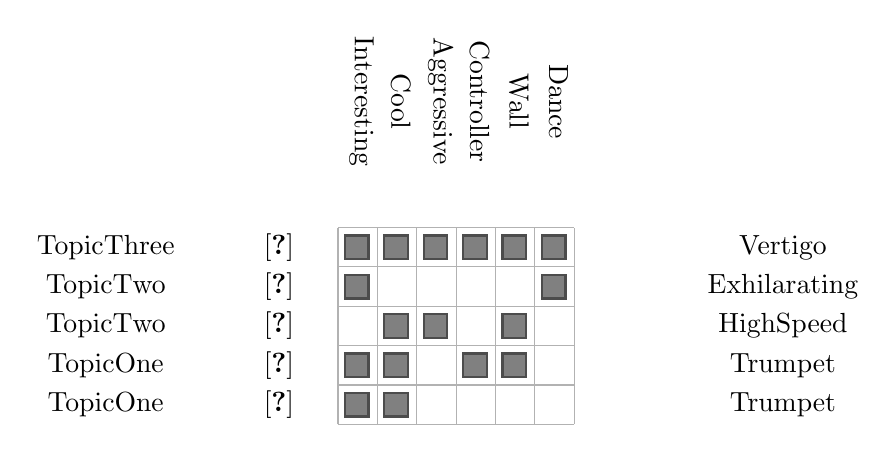
\begin{tikzpicture}[
	gridlines/.style={
		color=black!30,
		thin
	},
	featurebox/.style={
		rectangle,
		minimum size=3mm,
		draw=black!70,
		fill=black!50,
		thick
	}
]



\def\numfeatures{6} % needs to be updated manually
\def\featurenames{
	Interesting,
	Cool,
	Aggressive,
	Controller,
	Wall,
	Dance, % the last comma seems important to have
}


\def\numpapers{5} % needs to be updated manually
\def\papers{
	{
		\cite{ReferenceOne},
		TopicOne,
		{Interesting, Cool},
		Trumpet
	},
	{
		\cite{ReferenceTwo},
		TopicOne,
		{Interesting, Cool, Controller, Wall},
		Trumpet
	},
	{
		\cite{ReferenceOne},
		TopicTwo,
		{Cool, Aggressive, Wall},
		HighSpeed
	},
	{
		\cite{ReferenceOne},
		TopicTwo,
		{Interesting, Dance},
		Exhilarating
	},
	{
		\cite{ReferenceTwo},
		TopicThree,
		{Interesting, Cool, Aggressive, Controller, Wall, Dance},
		Vertigo
	}, % the last comma seems important to have
}






\def\gridstep{0.5}
\def\gridoffset{2.5}
\def\gridstepcm{\gridstep cm}
\def\gridoffsetcm{\gridoffset cm}

\def\gridwidth{\numfeatures*\gridstep cm}
\def\gridheight{\numpapers*\gridstep}

\draw[
	step=\gridstep,
	shift={(0.1+\gridstep*0.5,\gridstep*0.5)},
	gridlines
] (0,0) grid (\gridwidth,\gridheight);





\def\colcitation{1}
\def\coltopic{2}
\def\colfeature{3}
\def\colgenre{4}

\foreach \paper [count=\i] in \papers {
	\foreach \field [count=\col] in \paper {
		\ifx \col \coltopic
			\node at (-5.1+\gridoffset,\i*0.5) {{\field}};
		\fi

		\ifx \col \colcitation
			\node at (-2.9+\gridoffset,\i*0.5) {{\field}};
		\fi

		\ifx \col \colfeature % current = {1,0,1} feature list
			\foreach \hasfeature [count=\k] in \field {
				\foreach \feature [count=\featureindex] in \featurenames {
					\ifx \hasfeature \feature
						\node at (\gridoffset+\featureindex*\gridstepcm,\i*\gridstep) [featurebox] {};
					\fi
				}
			}
		\fi

		\ifx \col \colgenre
			\node at (0.5+\gridoffset+\numfeatures*\gridstep,\i*0.5) {{\field}};
		\fi
	}
}



\foreach \feature [count=\i] in \featurenames {
	\node [
		rotate=-90
	] at (0.15+\i*0.5,1.85+\numpapers*\gridstep) {\feature};
}



\end{tikzpicture}

\caption{Dimensions (columns) vs projects in past work (rows)....}
\label{figure:designspace}

\end{figure}


